% Part: model-theory
% Chapter: interpolation
% Section: separation

\documentclass[../../../include/open-logic-section]{subfiles}

\begin{document}

\olfileid{mod}{int}{sep}

\olsection{فصل الـ\printtoken{P}{sentence}}

نحتاج إلى شيء من التمهيد قبل الشروع في برهان مبرهنة الاستيفاء. مستوفية
$!A$ و$!B$ هي !!a{sentence}~$!C$ بحيث $!A \Entails !C$ و
$!C \Entails !B$. وبالمقابلة، تصح الأخيرة إذا وفقط إذا كان
$\lnot !B \Entails \lnot !C$. ويقال إن !!^a{sentence}~$!C$ بهذه
الخاصية \emph{تفصل} $!A$ عن $\lnot !B$. ومن ثم فإن إيجاد مستوفية لـ
$!A$ و$!B$ يكافئ إيجاد !!a{sentence} تفصل $!A$ عن $\lnot !B$.
وكثيرًا ما يكون من المفيد النظر في تعميم: جملة تفصل \emph{مجموعتين} من
الـ!!{sentence}s.

\begin{defn}
\emph{تفصل} جملة~$!C$ مجموعتي الجمل $\Gamma$ و$\Delta$ إذا وفقط إذا كان
$\Gamma \Entails !C$ و$\Delta \Entails \lnot !C$. وإذا لم توجد
!!{sentence} كهذه، كانت $\Gamma$ و$\Delta$ \emph{غير قابلتين للفصل}.
\end{defn}

تمثل أدناه علاقات الاحتواء بين فئات نماذج $\Gamma$ و$\Delta$ و$!C$:
\begin{figure}[h]
  \centering
  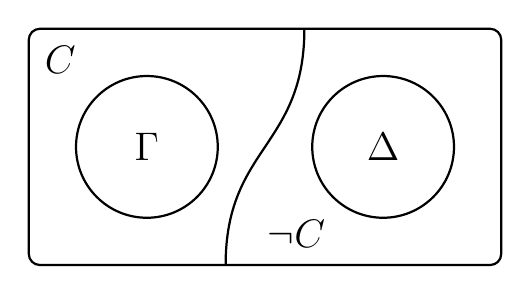
\begin{tikzpicture}[node distance=2cm, auto, thick]
    \draw [rounded corners] (0,0) -- (6,0) -- (6,3) -- (0,3) --  cycle;
    \draw (1.5,1.5) circle (0.9cm);
    \draw (4.5,1.5) circle (0.9cm);
    \path node at (1.5,1.5) {\Large $\Gamma$};
    \path node at (4.5,1.5) {\Large $\Delta$};
    \path node at (0.4,2.6) {\Large $\formula{C}$};
    \path node at (3.4,0.4) {\Large $\lnot \formula{C}$};
    \draw (2.5,0) .. controls (2.5,1.5) and (3.5,1.5) .. (3.5,3);
  \end{tikzpicture}
  \caption{$!C$ تفصل $\Gamma$ عن $\Delta$}
  \ollabel{fig:sep}
\end{figure}


\begin{lem}\ollabel{lem:sep1}
افترض أن $\Lang{L}_0$ هي اللغة التي تحتوي كل !!{constant} و!!{function}
و!!{predicate} (عدا~$\doteq$) يقع في $\Gamma$ و$\Delta$ \emph{معًا}،
ولتكن $\Lang{L}'_0$ ناتجة بإضافة عدد لا نهائي من الـ!!{constant}s الجديدة
$\Obj c_n$، حيث $n \ge 0$. إذا كانت $\Gamma$ و$\Delta$ غير قابلتين
للفصل في $\Lang{L}_0$، فهما غير قابلتين للفصل في $\Lang{L}'_0$ أيضًا.
\end{lem}

\begin{proof}
نسلك طريقًا غير مباشر: افترض طلبًا للتناقض أن $\Gamma$ و$\Delta$ قابلتان
للفصل في $\Lang{L}'_0$. عندئذ
$\Gamma \Entails \Subst{!C}{c}{x}$ و
$\Delta \Entails \lnot \Subst{!C}{c}{x}$ لبعض
$!C \in \Lang{L}_0$ (حيث $c$~!!{constant} جديد؛ وحالة احتواء $!C$ أكثر
من !!{constant} جديد واحد مماثلة). وبالتراص توجد مجموعتان جزئيتان
\emph{منتهيتان} $\Gamma_0$ من $\Gamma$ و$\Delta_0$ من $\Delta$ بحيث
$\Gamma_0 \Entails \Subst{!C}{c}{x}$ و
$\Delta_0 \Entails \lnot \Subst{!C}{c}{x}$. ولتكن $!G$ اقتران جميع
الـ!!{formula}s في $\Gamma_0$، و$!H$ اقتران جميع الـ!!{formula}s في
$\Delta_0$. عندئذ
\begin{align*}
  !G & \Entails \Subst{!C}{c}{x}, & !H  \Entails \lnot \Subst{!C}{c}{x}.
\end{align*}
من الأولى نحصل، بالتعميم، على $!G \Entails \lforall[x][!C]$، ومن
الثانية نحصل بالمقابلة على
$\Subst{!C}{c}{x} \Entails \lnot !H$، ومن ثم كذلك
$\lforall[x][!C] \Entails \lnot !H$. وتعطينا المقابلة مرة أخرى
$!H \Entails \lnot \lforall[x][!C]$. وبالرتابة:
\begin{align*}
  \Gamma &\Entails \lforall[x][!C], &
  \Delta & \Entails \lnot \lforall[x][!C],
\end{align*}
فتفصل $\lforall[x][!C]$~$\Gamma$ عن $\Delta$ في $\Lang{L}_0$.
\end{proof}

\begin{lem}\ollabel{lem:sep2}
افترض أن $\Gamma \cup \{ \lexists[x][!S] \}$ و$\Delta$ غير قابلتين
للفصل، وأن $c$~!!{constant} جديد لا يقع في $\Gamma$ أو $\Delta$ أو
$!S$. عندئذ تكون
$\Gamma \cup \{ \lexists[x][!S], \Subst{!S}{c}{x} \}$ و$\Delta$
غير قابلتين للفصل أيضًا.
\end{lem}

\begin{proof}
افترض طلبًا للتناقض أن $!C$ تفصل
$\Gamma \cup \{\lexists[x][!S], \Subst{!S}{c}{x}\}$ عن $\Delta$،
مع أن $\Gamma \cup \{\lexists[x][!S] \}$ و$\Delta$ غير قابلتين
للفصل. نميز حالتين:
\begin{enumerate}
\item لا يقع $c$ في $!C$: في هذه الحالة تكون
  $\Gamma \cup \{\lexists[x][!S], \lnot!C \}$ قابلة للإرضاء (وإلا
  لفصلت $!C$~$\Gamma \cup \{\lexists[x][!S] \}$ عن $\Delta$).
  وتظل كذلك إذا أضيفت $\Subst{!S}{c}{x}$، ومن ثم لا تفصل $!C$ في
  النهاية $\Gamma \cup \{ \lexists[x][!S], \Subst{!S}{c}{x} \}$
  عن $\Delta$.
\item يقع $c$ في $!C$، فتكون $!C$ على الصورة
  $\Subst{!C}{c}{x}$. عندئذ لدينا
  \[
  \Gamma \cup \{ \lexists[x][!S], \Subst{!S}{c}{x}\} \Entails \Subst{!C}{c}{x},
  \]
  ومنه $\Gamma, \lexists[x][!S] \Entails \lforall[x][(!S \lif !C)]$
  بمبرهنة الاستنباط والتعميم، وأخيرًا
  $\Gamma \cup \{ \lexists[x][!S] \} \Entails \lexists[x][!C]$.
  ومن جهة أخرى، $\Delta \Entails \lnot \Subst{!C}{c}{x}$، ومن ثم
  بالتعميم $\Delta \Entails \lnot \lexists[x][!C]$. وهكذا تكون
  $\Gamma \cup \{\lexists[x][!S] \}$ و$\Delta$ قابلتين للفصل، وهو
  تناقض.
\end{enumerate}
\end{proof}

\end{document}
